\documentclass{beamer}
\usetheme[pageofpages=of,% String used between the current page and the
                         % total page count.
          bullet=circle,% Use circles instead of squares for bullets.
          titleline=true,% Show a line below the frame title.
          alternativetitlepage=true,% Use the fancy title page.
       %   titlepagelogo=logo-polito,% Logo for the first page.
       %   watermark=watermark-polito,% Watermark used in every page.
       %   watermarkheight=100px,% Height of the watermark.
       %   watermarkheightmult=4,% The watermark image is 4 times bigger
                                % than watermarkheight.
          ]{Torino}

\setbeamertemplate{footline}{
  \begin{beamercolorbox}[wd=\paperwidth,ht=1ex,dp=1ex]{footline}
    \vspace{5pt} \hspace{1em} \insertframenumber/\inserttotalframenumber
  \end{beamercolorbox}
}

\author{Brendon J. Brewer}
\title{STATS 331 -- Introduction to Bayesian Statistics}
\institute{The University of Auckland}
\date{}


\linespread{1.3}
\usepackage{minted}
\usepackage[utf8]{inputenc}
\usepackage{dsfont}
\newcommand{\given}{\,|\,}


\begin{document}

\frame{\titlepage}

\begin{frame}
\centering
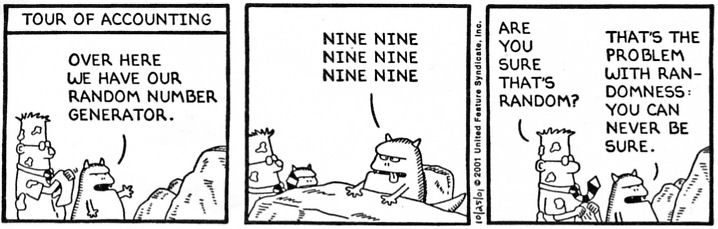
\includegraphics[width=0.8\textwidth]{images/dilbert.jpg}

\end{frame}



\begin{frame}
\centering
\large
Bayesian Linear Regression

\end{frame}


\begin{frame}
\frametitle{Models}
\begin{itemize}
\item We have seen most of the fundamental principles that we will need
throughtout the course.\pause
\item From now on, most of what we will study are particular `models'
for common data analysis situations.\pause
\item We will start with simple linear regression.
\end{itemize}

\end{frame}



\begin{frame}
\frametitle{Road Sign Data}
\centering
\includegraphics[width=0.8\textwidth]{images/road_data.pdf}
\end{frame}


\begin{frame}[fragile]
\frametitle{Classical Least Squares Regression in R}
\tiny
\begin{minted}{r}
> data = read.table("road.txt")
> result = lm(data[, 2] ~ data[, 1])
> summary(result)

Call:
lm(formula = data[, 2] ~ data[, 1])

Residuals:
    Min      1Q  Median      3Q     Max 
-78.231 -41.710   7.646  33.552 108.831 

Coefficients:
            Estimate Std. Error t value Pr(>|t|)    
(Intercept) 576.6819    23.4709  24.570  < 2e-16 ***
data[, 1]    -3.0068     0.4243  -7.086 1.04e-07 ***
---
Signif. codes:  0 ‘***’ 0.001 ‘**’ 0.01 ‘*’ 0.05 ‘.’ 0.1 ‘ ’ 1

Residual standard error: 49.76 on 28 degrees of freedom
Multiple R-squared:  0.642,	Adjusted R-squared:  0.6292 
F-statistic: 50.21 on 1 and 28 DF,  p-value: 1.041e-07
\end{minted}

\end{frame}

\begin{frame}[fragile]
\frametitle{Classical Least Squares Regression in R}
\begin{minted}{r}
plot(data[, 1], data[, 2])
abline(result)
\end{minted}

\end{frame}

\begin{frame}
\frametitle{Classical Least Squares Regression in R}
\centering
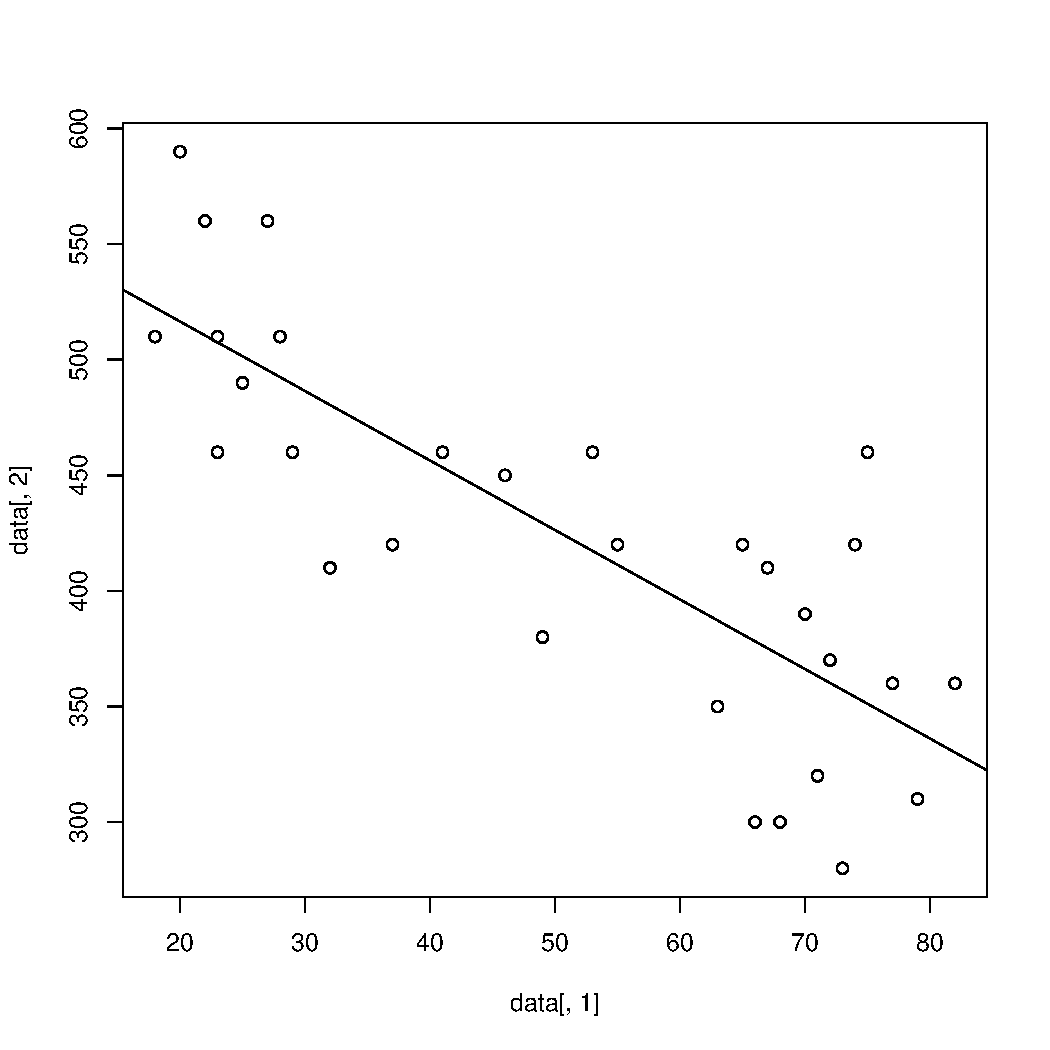
\includegraphics[width=0.6\textwidth]{images/road_lm.pdf}
\end{frame}


\begin{frame}
\frametitle{Least Squares}
In classical regression you fit a line of the form
\begin{align}
y &= \beta_0 + \beta_1 x
\end{align}
by minimising the sum of squared residuals
\begin{align}
\sum_{i=1}^N \left(y_i - (\beta_0 + \beta_1 x_i)\right)^2.
\end{align}
\pause
From the estimated $\beta_0$ and $\beta_1$ values
you can predict the value of $y$ at any other value of $x$.

\end{frame}


\begin{frame}
\frametitle{Bayesian Approach}

\begin{itemize}
\item We will use Bayes' theorem to obtain the {\bf joint}
posterior distribution for three unknown parameters
$\beta_0$, $\beta_1$, and $\sigma$.\pause
\item The parameter $\sigma$ was not mentioned before
but describes the typical degree of scatter about the line.\pause
\item Our data is the `response variable'
$\{y_1, ..., y_N\}$ and the explanatory variable
$\{x_1, ..., x_N\}$ is considered part of the prior information.
\end{itemize}

\end{frame}


\begin{frame}
\frametitle{Bayesian Approach}

\begin{itemize}
\item We will need a prior distribution $p(\beta_0, \beta_1, \sigma)$,
and a sampling distribution $p(y_1, ..., y_N \given \beta_0, \beta_1, \sigma)$.\pause
\item For the sampling distribution, imagine knowing the parameters but not
the data --- what distribution would you write down?\pause
\item The standard assumption for the sampling distribution is
to put a normal distribution around what the straight line would predict:
\end{itemize}
\begin{align}
y_i \given \beta_0, \beta_1, \sigma &\sim \textnormal{Normal}
    \left(\beta_0 + \beta_1 x_i, \sigma^2\right).
\end{align}


\end{frame}


\begin{frame}
\frametitle{Bayesian Approach: Analytical}
This problem can actually be solved analytically, but it's pretty hardcore.
We can get a bit of insight by writing down Bayes' rule:
\begin{align}
p(\beta_0, \beta_1, \sigma \given \boldsymbol{y})
    &\propto p(\beta_0, \beta_1, \sigma)p(\boldsymbol{y} \given \beta_0, \beta_1, \sigma)\\
    &\propto p(\beta_0, \beta_1, \sigma)
        \prod_{i=1}^N \frac{1}{\sigma\sqrt{2\pi}}
            \exp\left[-\frac{1}{2\sigma^2}\left(y_i - (\beta_0 + \beta_1 x_i)\right)^2\right] \\
    &\propto p(\beta_0, \beta_1, \sigma)
        \sigma^{-N}
            \exp\left[-\frac{1}{2\sigma^2}\sum_{i=1}^N\left(y_i - (\beta_0 + \beta_1 x_i)\right)^2\right]
\end{align}

\end{frame}




\begin{frame}
\frametitle{Bayesian Approach: Analytical}
The sum of squared residuals has appeared in the likelihood function!
If we have a uniform prior, the posterior mode is in fact the least squares
estimate.\pause

We should not expect large quantitative differences between Bayesian and
classical regression results if our priors are wide and we have the standard
assumptions. We will still implement it with these assumptions, but we will
also look at varying the assumptions later.
\end{frame}


\begin{frame}[fragile]
\frametitle{Bayesian Approach: JAGS Model}

\footnotesize
\begin{minted}{r}
model
{
    beta0 ~ dunif(-1000, 1000) # Casual wide priors
    beta1 ~ dunif(-1000, 1000) # These might not always be appropriate
    log_sigma ~ dunif(-10, 10) # Log-uniform prior for sigma
    sigma <- exp(log_sigma)

    for(i in 1:length(y)) # In case N is not provided with the data
    {
        y[i] ~ dnorm(beta0 + beta1*x[i], 1/sigma^2)
    }
}
\end{minted}

\end{frame}

\begin{frame}[fragile]
\frametitle{Bayesian Approach: Deterministic Nodes}
It is possible to write the sampling distribution in this alternative form,
where the regression line has been defined separately as its own node.
\begin{minted}{r}
for(i in 1:length(y))
{
    mu[i] <- beta0 + beta1*x[i]
    y[i] ~ dnorm(mu[i], 1/sigma^2)
}
\end{minted}


\end{frame}


\begin{frame}[fragile]
\frametitle{Other Casual Wide Priors}
Statisticians will often use wide priors that are conjugate priors, as this
can speed up the performance of JAGS. However, I don't really like these
because the meaning is more obscure.
\begin{minted}{r}
beta0 ~ dnorm(0, 1/1000^2)
beta1 ~ dnorm(0, 1/1000^2)
sigma ~ dgamma(0.001, 0.001)
\end{minted}

I will sometimes use the \mintinline{r}{dnorm()} versions but do not recommend
the \mintinline{r}{dgamma()} as it is dangerous (it is more informative than
it appears to be).
\end{frame}


\begin{frame}[fragile]
\frametitle{Running JAGS}
\large
Let's run JAGS with this model and inspect the results.
\end{frame}


\begin{frame}[fragile]
\frametitle{Plotting Lines Through the Data}
It is useful to visualise the fit.
\begin{minted}{r}
x = seq(0.0, 100.0, by=0.1)
plot(data$x, data$y, xlim=c(0, 100))
rows = sample(1:nrow(results), 100)
for(row in rows)
{
    y = results$beta0[row] + results$beta1[row]*x
    lines(x, y, col=rgb(0, 0, 0, 0.1))
}
\end{minted}

\end{frame}

\begin{frame}
\frametitle{Plotting Lines Through the Data}
\begin{center}
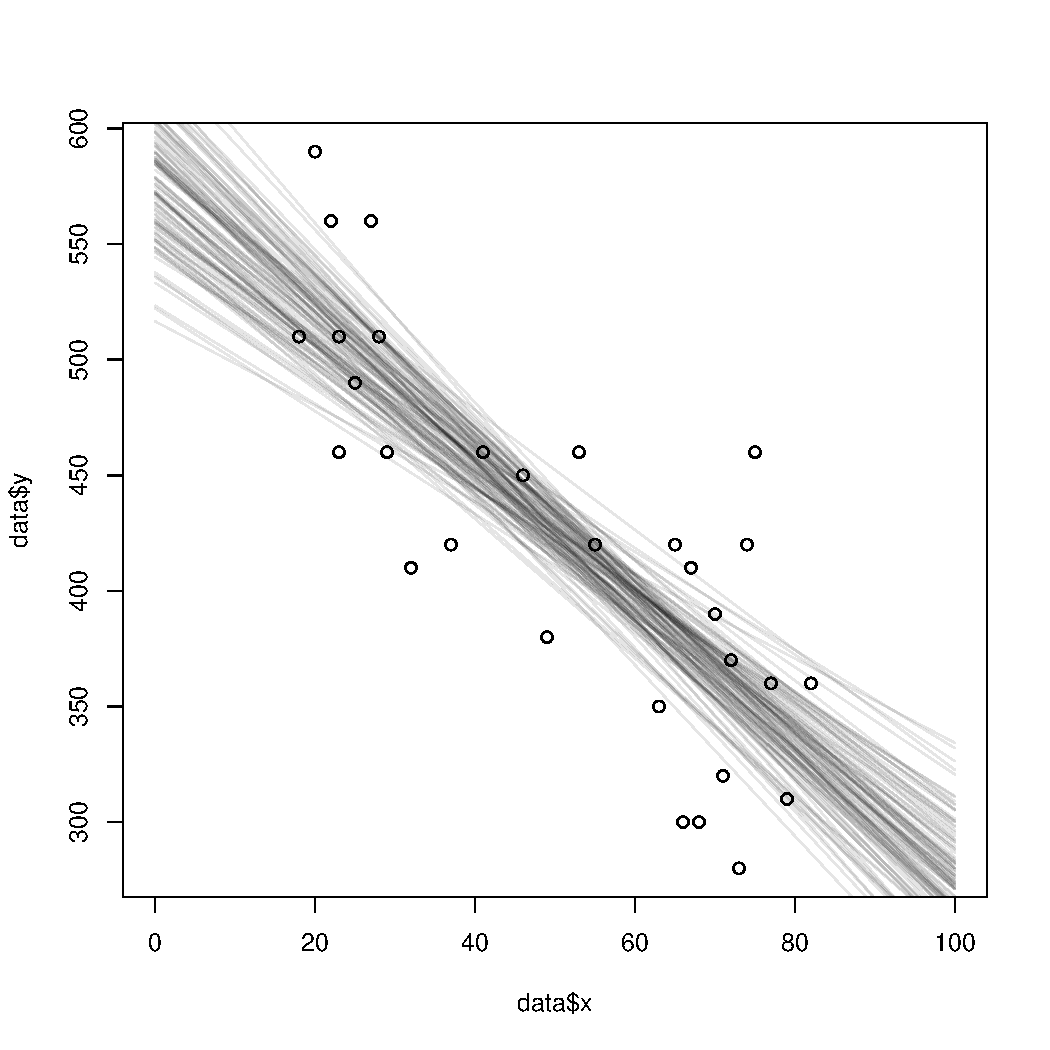
\includegraphics[width=0.55\textwidth]{images/road_lines.pdf}
\end{center}
\end{frame}



\begin{frame}[fragile]
\frametitle{Plotting Posterior Distributions}
We can get some idea of what the 3-D joint posterior distribution is like
by plotting a `corner plot', which is a set of 2-D marginal distributions.
They don't look amazing, but you can do a basic one in R with the
\mintinline{r}{pairs()} function. Here, I'm shrinking the circles with
\mintinline{r}{cex=0.1} so they are basically dots.

\begin{minted}{r}
pairs(results, cex=0.1)
\end{minted}

\end{frame}


\begin{frame}
\frametitle{Corner Plot}
\begin{center}
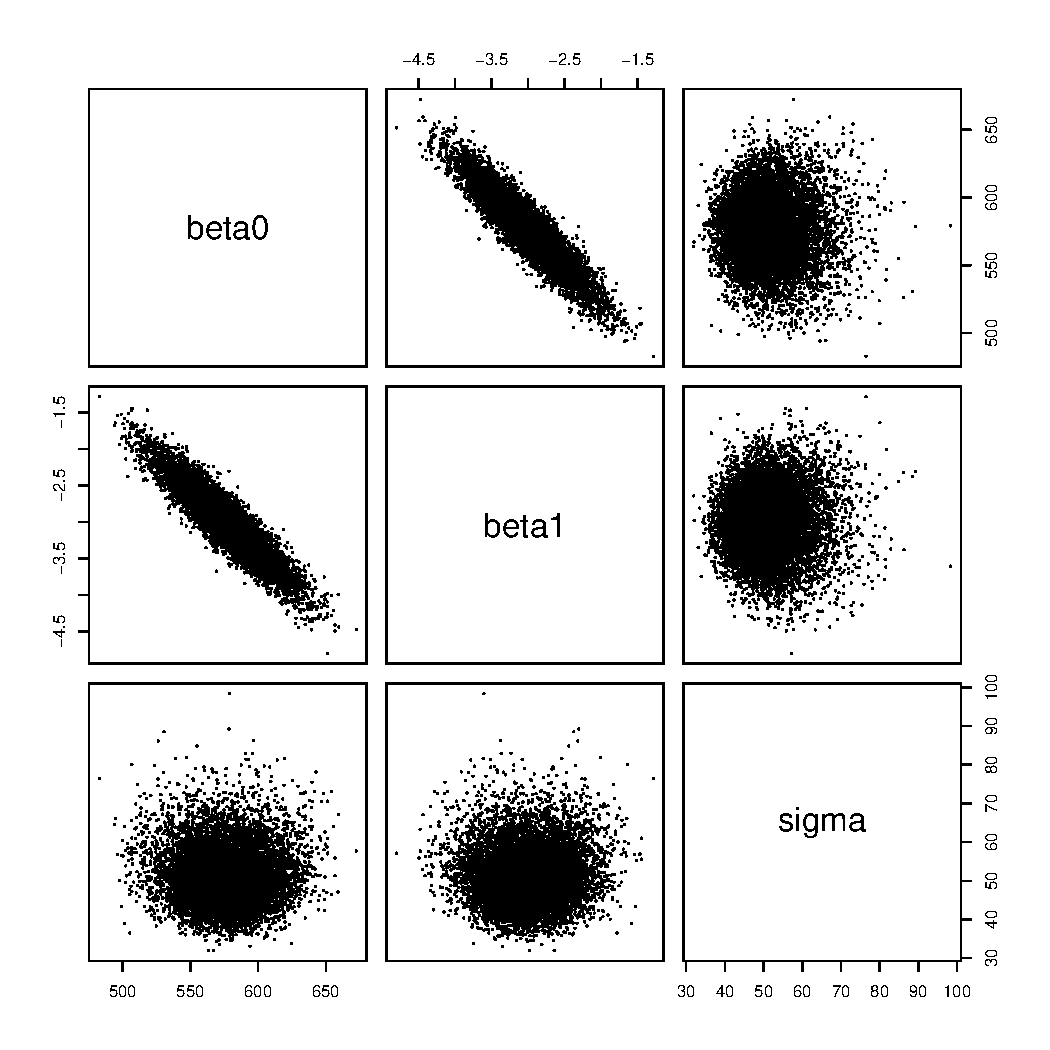
\includegraphics[width=0.55\textwidth]{images/road_corner.pdf}
\end{center}
\end{frame}


\begin{frame}
\frametitle{Dependence in the Posterior Distribution}
We can see some dependence between the parameters in the posterior distribution,
especially between $\beta_0$ and $\beta_1$. If $\beta_0$ is increased, then
in order to still fit the data, $\beta_1$ must be decreased.\pause

Sometimes, dependence in the posterior distribution is so strong that it
affects the efficiency of the MCMC (when using the methods JAGS uses,
which update one parameter at a time while keeping the others fixed).
\end{frame}



\begin{frame}[fragile]
\frametitle{Centering Explanatory Variables}
Some of the reason for the dependence is because all of the observations
are far from $x=0$, so for a line to fit through the observations, it must
exactly `hit' the cloud of points. This effect can be reduced by {\bf centering}
the explanatory variables:

\begin{minted}{r}
mu[i] <- beta0 + beta1*(x[i] - mean(x))
\end{minted}
\end{frame}

\begin{frame}
\frametitle{Corner Plot}
\begin{center}
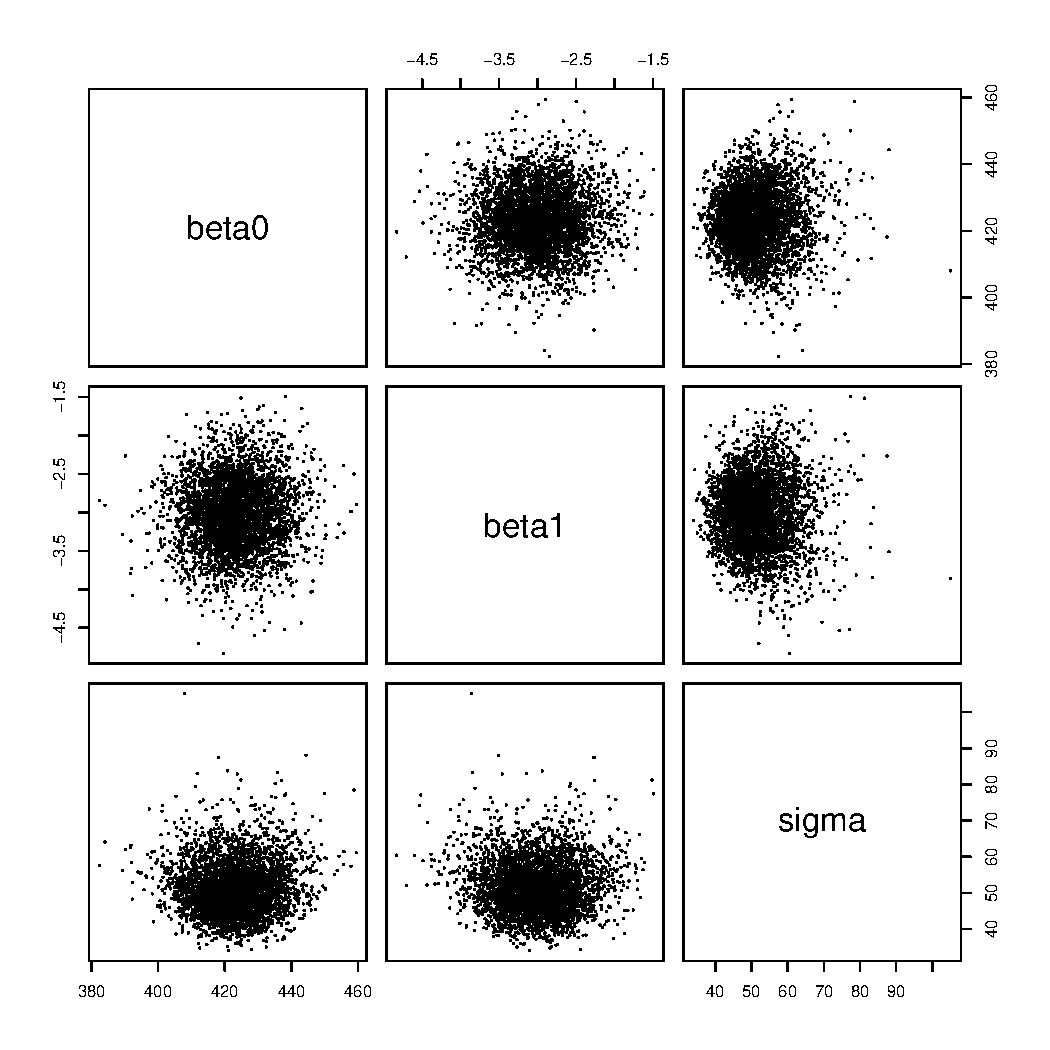
\includegraphics[width=0.55\textwidth]{images/road_corner2.pdf}
\end{center}
\end{frame}

\begin{frame}[fragile]
\frametitle{Centering Explanatory Variables}
Note: Centering changes the meaning of $\beta_0$. Instead of being the typical
value of the response variable $y$ when $x=0$, it is the typical value of
$y$ when $x=(x_1 + ... + x_N)/N$.\pause

Also, the priors are not exactly equivalent, but this doesn't usually matter.
\end{frame}

\begin{frame}
\frametitle{Prediction in JAGS}
\begin{itemize}
\item If we knew the perameters, we could extrapolate the line to predict
what will happen to $y$ when $x=x_{\rm new}$.\pause
\item You should create a normal distribution around this with standard deviation
$\sigma$.\pause
\item However, $\sigma$ is unknown, as are $\beta_0$ and $\beta_1$.
\end{itemize}
\end{frame}


\begin{frame}
\frametitle{Prediction in JAGS}
The Bayesian procedure to make such a prediction, taking into account all
uncertainties, would be:
\begin{itemize}
\item Loop over the posterior samples.\pause
\item For each possible value of the parameters,
extrapolate the line using $\beta_0$ and $\beta_1$, and add noise with sd
given by $\sigma$.\pause
\item Look at the distribution of $y_{\rm new}$ that you get.\pause
\end{itemize}
This can be done manually, but it's even easier to do it in JAGS.

\end{frame}



\begin{frame}[fragile]
\frametitle{Prediction in JAGS}
Simply add ``one extra data point'' whose sampling distribution is (usually)
the same, but whose value is unobserved (not provided with the data).
In regression models, we need to put in the value of the explanatory variable:
\begin{minted}{r}
for(i in 1:length(y))
{
    y[i] ~ dnorm(beta0 + beta1*x[i], 1/sigma^2)
}
y_new ~ dnorm(beta0 + beta1*100, 1/sigma^2)
\end{minted}
\end{frame}


\end{document}

